\section{Application avec Python sur les ports GPIO}

\subsection{Qu'est ce que le GPIO ?}

GPIO est l'acronyme de \emph{General Purpose Input Output}.

C'est la série de broches situé sur un côté du Raspberry. Sa taille a varié entre le premier Raspberry et les suivants. On a gagné quelques broches.

Sur la figure \ref{img_gpio}, du site element14, est représenté le GPIO pour le Raspberry Pi 3, il faut que vous cherchiez sur internet celui qui correspond à votre modèle de Pi si nécessaire.

\begin{center}
\begin{figure}
	\scalebox{0.5}{
	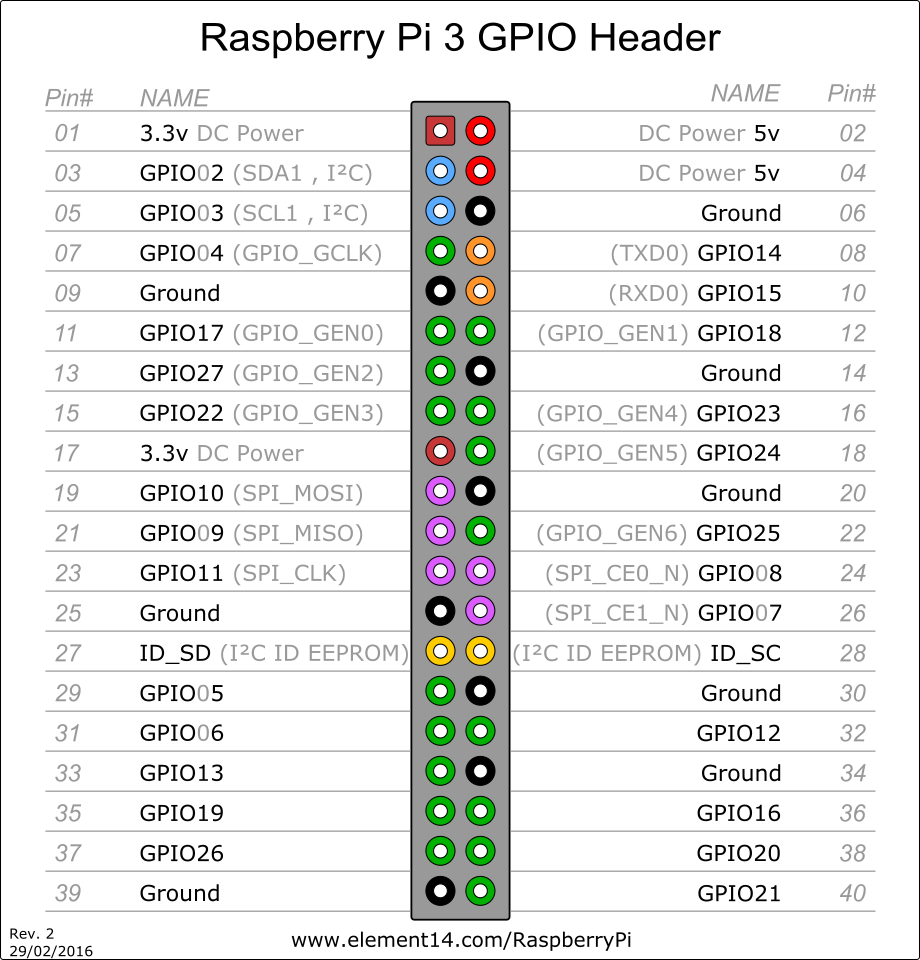
\includegraphics{images/gpio}
	}
	\caption{Le GPIO du Raspberry Pi 3}
	\label{img_gpio}
\end{figure}
\end{center}

Vous pouvez remarquer qu'il y a des alimentations de 3,3V et de 5V (pin 01, 02, 04, 17) selon les périphériques que vous voulez brancher. Et Il y a des masses \emph{Ground}.

Les autres broches sont sur du courants de 3,3V. Le courant en sortie peut varier de 2 à 16mA. 

Le GPIO permet de soit de contrôler soi même des éléments électroniques soit de mettre des extensions (HAT) pour avoir des périphériques. Vous en aurez à disposition le jour de l'atelier en petit nombre.

Le plus simple pour gérer ces sorties est le langage Python. Une bibliothèque Python est fourni pour contrôler le GPIO et aussi les périphériques qu'on branche dessus (le plus souvent).

Sinon vous avez la possibilité de contrôler le GPIO via un programme en C.

Pour installer les paquets nécessaires en python il faut faire~:
\begin{verbatim}
$sudo apt-get install python-pip
$sudo pip install RPi.GPIO
\end{verbatim}


\subsection{Eclairer une diode}

C'est la partie que je maitrise pas trop, c'est la partie électronique.

Pour allumer une diode, il faut mettre la résistance adéquate pour ne pas griller la diode. Pour une tension de 3,3V et avec une diode qui fait baisser la tension de 0,7V il faut absorber $3,3-0,7=2,6V$. Avec la loi d'Ohms, $U=R/I$, on calcule pour un courant de 5mA la résistance nécessaire~: $2,6/(5/1000)=520 ohms$. La résistance la plus proche est de 570 ohms. 

Il faut chercher la résistance qui va bien. Installer fil, diode et résistance sur la breadboard.

Ensuite le programme Python est assez simple~:
\begin{verbatim}
import RPi.GPIO as GPIO
import time

# Activer la bonne numérotation des pins
GPIO.setmode(GPIO.BCM)

# Si la diode est branché sur la pin 18.
# 1) activer la broche en sortie de courant
GPIO.setup(18, GPIO.OUT)
# 2) activer la diode
GPIO.output(18, GPIO.HIGH)

# Attendre 2 secondes
time.sleep(2)

# Eteindre la diode
GPIO.output(18, GPIO.LOW)
\end{verbatim} 

C'est tout\dots

Pour faire un programme qui va faire clignoter indéfiniment la diode.

\begin{verbatim}
import Rpi.GPIO as GPIO
import time

GPIO.setmode(GPIO.BCM)
GPIO.setup(18, GPIO.OUT)

while TRUE:
    GPIO.output(18, GPIO.HIGH)
   time.sleep(1)
   GPIO.output(18, GPIO.LOW)
   time.sleep(1)
\end{verbatim} 

Attention en l'arrêtant avec controle+C vous allez laisser la broche dans un état ambigu.

Il vaut mieux quitter proprement~:

\begin{verbatim}
import RPi.GPIO as GPIO
import time

GPIO.setmode(GPIO.BCM)
GPIO.setup(18, GPIO.OUT)

while TRUE:
    try:
        GPIO.output(18, GPIO.HIGH)
        time.sleep(1)
        GPIO.output(18, GPIO.LOW)
        time.sleep(1)
    except KeyboardInterrupt:
        break

GPIO.cleanup()
\end{verbatim}

 \subsection{PiFaceCAD}
 
 Le PiFace est une carte avec un afficheur deux lignes 16 caractères, des boutons poussoirs et un un capteur infra-rouge.
 
Pour l'utiliser il faut activer la sortie SPI dans `raspi-config', redémarrer puis installer le paquet python-piface.

\begin{verbatim}
$sudo apt-get install python-pifacecad
\end{verbatim}
 
 \begin{verbatim}
import pifacecad
import time
import netifaces as ni

# Trouver l'adresse IP
ni.ifaddresses('eth0')
ip = ni.ifaddresses('eth0')[2][0]['addr']

# Allumer le PiFace
cad = pifacecad.PiFaceCAD()
cad.lcd.backlight_on()
cad.lcd.clear()

# Afficher au premier caractère sur la première ligne
cad.lcd.set_cursor(1, 0)        
cad.lcd.write(`Hello World')

cad.lcd.set_cursor(1, 1)        
cad.lcd.write(ip)

sleep(5)

cad.lcd.backlight_off()

\end{verbatim}

Pour utiliser les boutons poussoirs, on crée un processus qui va surveiller et faire un ``goto'' dans une fonction pour traiter l'information.

\begin{verbatim}
import pifacecad
import time

def update_pin_text(event):
    cad.lcd.clear()   
     
    pin = event.pin_num + 0
    
    cad.lcd.set_cursor(1, 1)        
    cad.lcd.write(pin)
    
    sleep(0.5)
    
    return()    

listener = pifacecad.SwitchEventListener(chip=cad)

for i in range(8):
    listener.register(i, pifacecad.IODIR_FALLING_EDGE, update_pin_text)

listener.activate()

while True:
    try:
        pass
    except:
        break
\end{verbatim}

\subsection{Sense HAT}

Il s'agit d'un ``chapeau'' ayant comme capteur~:
\begin{itemize}
    \item Gyroscope
    \item Accélèrometre
    \item Magnetomètre
    \item Capteur de temperature
    \item Capteur d'humidité
    \item Capteur de pression barometric
\end{itemize}

Il possède aussi un affichage avec une matrice de 8x8 en RGB.

Il est célèbre pour avoir voyagé dans l'espace.

Pour installer le package il faut faire~:
\begin{verbatim}
$sudo apt-get install python-sense-hat
\end{verbatim}

Ci-dessous un script pour stocker dans un fichier l'humidité et la température que j'utilise chez moi.

\begin{verbatim}
#!/usr/bin/python
import sys
import os
import datetime

from sense_hat import SenseHat

sense = SenseHat()
humidity = sense.get_humidity()
print("Humidity: %s %%rH" % humidity)

temp = sense.get_temperature()
print("Temperature: %s C" % temp)

pressure = sense.get_pressure()
print("Pressure: %s Millibars" % pressure)

dateheure = datetime.datetime.now().strftime("%Y/%m/%d %H:%M:%S")

fh = open("temp.csv", 'a')
fh.write("%s;%s;%s;%s\n" % (dateheure,temp,humidity,pressure))
\end{verbatim}


